\documentclass[12pt]{article}
\usepackage[czech]{babel}
\usepackage[utf8]{inputenc}
\usepackage[IL2]{fontenc}
\usepackage{wrapfig}
\usepackage{graphicx}
\usepackage{amsmath}
\usepackage{scrextend}
\usepackage{cprotect}
\usepackage{float}
\usepackage{hyperref}
\usepackage{indentfirst}
\newcommand{\htmltag}[1]{%
	\scalebox{.6}[1]{$<$}{\ttfamily#1}\scalebox{.6}[1]{$>$}%
}

\begin{document}
\pagenumbering{gobble} %bez cisel
\begin{titlepage}
\centerline{
\includegraphics[width=10cm]{img/logo.jpg}}
\begin{center}
\vspace{30px}
{\Huge
\textbf{Semestrální práce KIV/BIT}\\
\vspace{1cm}
}
{\Large
\textbf{Implementace šifry AES}\\
}
\vspace{1cm}
{\large
Pavel Třeštík\\
}
{\normalsize
A17B0380P
}
\end{center}
\vspace{\fill}
\hfill
\begin{minipage}[t]{7cm}
\flushright
\today
\end{minipage}
\end{titlepage}

\tableofcontents
\newpage
\pagenumbering{arabic} %
%
% Zadání
%
\section{Zadání}
Úkolem je implementovat symetrickou blokovou šifru AES. Práce musí splňovat
následující podmínky.
\begin{itemize}
	\item Výsledek bude v hexadecimálním formátu.
	\item Použití šifrovacího módu ECB, tzn. aplikovat šifrovací algoritmus
		přímo na vstupní data. Inicializační vektor není potřeba.
		Dle nutnosti bude poslední blok dat zarovnán nulami z prava.
	\item Velikost bloku a klíče bude 128 bitů (16 Bytů). Klíč může zvolit
		uživatel
	\sloppy	\item Testovaní bude provedeno na poskytnutých souborech \textbf{Shea.jpg}
		a\,\textbf{message.txt} s klíčem \textbf{josefvencasladek}
\end{itemize}
%
% Analýza problému
%
\pagebreak
%
\section{Princip šifry AES}
Jedná se o symetrickou blokovou šifru. To znamená, že vstupní data jsou
šifrována po blocích a jsou šifrována i dešifrována pomocí stejného klíče.

Šifrování se provádí nad blokem dat, pro který se provádí několik transformací
v určitém počtu kol. Velikost bloku je shodná s velikostí klíče. Podle velikosti
klíče (bloku) je potom určen počet kol, kolikrát se provedou transformace. Pro
náš algoritmus je velikost klíče 128 bitů a počet kol pro tuto velikost je 10.

Algoritmus se potom skládá ze 4 částí, jejichž podrobnější vysvětlení následuje:
\begin{enumerate}
	\item \texttt{KeyExpansion} -- rozšíření klíče pomocí "Rijndael's key
		schedule". Jedná se o algoritmus, který vypočte nový klíč pro
		každé kolo AES šifrování. Každý nový klíč je odvozen z
		předchozího a úplně první klíč je klíč zvolen k šifrování.
		Pro jednotlivé klíče je potom využíván výraz \textbf{round key}.
	\item \texttt{AddRoundKey} -- aplikování prvního \textbf{round key} na
		blok dat, které budou šifrovány, před zahájením transformací.
	\item \texttt{9 kol transformací}:
		\begin{enumerate}
			\item \texttt{SubBytes} -- nahradí každý Byte stavu za 
				odpovídající Byte ve vyhledávací tabulce.
			\item \texttt{ShiftRows} -- posune pořadí prvků v
				řádkách.
			\item \texttt{MixColumns} -- kombinuje Byty ve sloupcích
				a výsledkem je sloupec jiných Bytů.
			\item \texttt{AddRoundKey} -- aplikování 
				\textbf{round key} pro dané kolo.
		\end{enumerate}
	\item \texttt{Poslední (10.) kolo transformací}:
		\begin{enumerate}
			\item \texttt{SubBytes}	
			\item \texttt{ShiftRows}
			\item \texttt{AddRoundKey}
		\end{enumerate}
		Jedná se o stále stejné transformace jako v kolech 1-9, ale už
		bez provedení kroku \texttt{MixColumns}. Tento krok je
		vynechán, aby mělo šifrování a\,dešifrování podobnější
		strukturu a také proto, že síla šifry už se nezmění i bez
		provedení tohoto kroku.
\end{enumerate}
%
\subsection{KeyExpansion}
Klíč je pro každé kolo šifrování jiný. Tyto klíče mohou být předem vygenerovány
pro všechna kola následujícím způsobem:
\begin{figure} [ht]
	\centering
	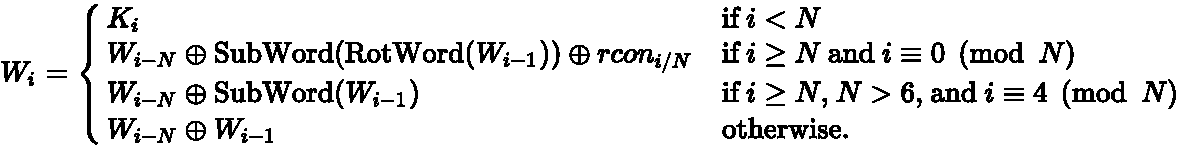
\includegraphics[width=\textwidth]{img/key_expansion_schedule.pdf}
	\caption{Způsob generování následujícího klíče}
	Zdroj: \url{https://en.wikipedia.org/wiki/AES\_key\_schedule}
	\label{fig:key_exp_schedule}
\end{figure}

\noindent\texttt{\textbf{$N$}} -- počet 32-bitových slov v klíči\\
\texttt{\textbf{$K_{i}$}} -- i-té slovo šifrovacího klíče\\
\texttt{\textbf{$W_{i}$}} -- i-té slovo generovaného klíče\\

Z Obrázku \ref{fig:key_exp_schedule} lze vidět, že se při generování slov klíče
používají funkce \texttt{SubWord} a \texttt{RotWord} a konstanta \texttt{rcon}.\\

\noindent\texttt{SubWord} -- jedná se v podstatě o \texttt{SubBytes} použité na
			Byty slova.\\
\texttt{RotWord} -- posune slovo o pozici doleva.\\
\indent\texttt{RotWord$[b_0 b_1 b_2 b_3]$ = $[b_1 b_2 b_3 b_0]$}\\
\texttt{rcon} -- může být spočítáno následujícím způsobem (viz Obrázek \ref{fig:key_exp_rc}).\\
\begin{figure} [ht]
	\centering
	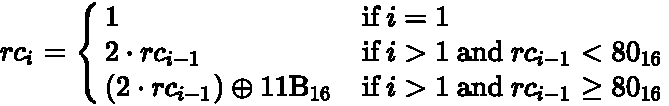
\includegraphics[width=\textwidth]{img/key_expansion_rc.pdf}
	\caption{Počítání konstanty rcon}
	Zdroj: \url{https://en.wikipedia.org/wiki/AES\_key\_schedule}
	\label{fig:key_exp_rc}
\end{figure}

\noindent\texttt{\textbf{$rc_i$}} -- první Byte slova klíče generovaného pro
					i-té kolo.\\
\texttt{\textbf{$i$}} -- i-té kolo\\
\pagebreak
%
\subsection{AddRoundKey}
Každý Byte bloku je nahrazen výsledkem operace XOR nad původním Bytem pozice a
odpovídajícím Bytem klíče pro dané kolo.

Na příklad 7-mý Byte bloku je výsledkem XOR mezi 7-mým Bytem bloku a 7-mým Bytem
klíče pro dané kolo.
%
\subsection{SubBytes}
Nahradí každý Byte bloku za odpovídající hodnotu ve vyhledávací tabulce. Jedná
se o "\textbf{Rijndael S-box}" (dále jen \textbf{S-box}) substituční tabulku.
Hodnota nahrazovaného Bytu se použije jako hodnota klíče (indexu) v 
\textbf{S-box} a nahradí Byte za hodnotu nacházející se na této pozici.

\textbf{S-box} může být vygenerován pomocí jednoduchého algoritmu, ale ten
jsem se rozhodl v rámci této semestrální práce neimplementovat.
%
\subsection{ShiftRows}
\noindent První řádku nemění.\footnote{Blok uvažujeme jako matici 4x4 pro náš
	16 Bytový blok}\\
Pro druhou řádku posune každý Byte o 1 do leva.\\
Pro třetí řádku posune každý Byte o 2 do leva.\\
Pro čtvrtou řádku posune každý Byte o 3 do leva.\\
%
\subsection{MixColumns}
Transformuje prvky tak, že vynásobí sloupec bloku konstantní maticí a\,výsledkem
je nový sloupec. Sloupec je násoben maticí:
\begin{equation*}
	\begin{bmatrix}
		2 & 3 & 1 & 1\\
		1 & 2 & 3 & 1\\
		1 & 1 & 2 & 3\\
		3 & 1 & 1 & 2
	\end{bmatrix}
\end{equation*}
%
\pagebreak
%
\subsection{Zdroje}
\subsubsection{Wikipedia}
\begin{itemize}
	\item Advanced Encryption Standard\\
		\sloppy
		\url{https://en.wikipedia.org/wiki/Advanced\_Encryption
		\_Standard}
	\item Rijndael S-box\\
		\url{https://en.wikipedia.org/wiki/Rijndael\_S-box}
	\item AES key schedule\\
		\url{https://en.wikipedia.org/wiki/AES\_key\_schedule}
	\item Rijndael MixColumns\\
		\url{https://en.wikipedia.org/wiki/Rijndael\_MixColumns}
	\item Finite field arithmetic\\
		\url{https://en.wikipedia.org/wiki/Finite\_field\_arithmetic}
\end{itemize}
\subsubsection{GitHub}
\begin{itemize}
	\item GitHub projekt uživatele kokke\\
		\url{https://github.com/kokke/tiny-AES-c}
	\item GitHub projekt uživatele dhuertas\\
		\url{https://github.com/dhuertas/AES}
\end{itemize}
\subsubsection{Jiné}
\begin{itemize}
	\item Příklad AES šifry\\
		\url{https://kavaliro.com/wp-content/uploads/2014/03/AES.pdf}
	\item Why is MixColumns omitted from the last round of AES?\\
		\sloppy
		\url{https://crypto.stackexchange.com/questions/1346/why
		-is-mixcolumns-omitted-from-the-last-round-of-aes}
\end{itemize}
%
% Implementace
%
\section{Implementace}
Práci jsem se rozhodl implementovat v jazyce C. Jazyk jsem si vybral především
proto, že se velká část činností provádí lépe na nižší úrovni a také pro
jeho rychlost.
\subsection{Moduly}
Projekt má pouze dva moduly. Modul šifrovacího algoritmu \texttt{aes.c}
(a\,příslušný header file) a modul obsluhy \texttt{main.c}.
\subsection{aes.c}
\subsubsection{Důležité konstanty}
\noindent\texttt{const u\_char Rcon[11]} -- rcon konstanty pro generování
\textbf{round key}\footnote{u\_char je typedef pro unsigned char, který
	jsem používal jako 1B strukturu}\\
\texttt{const u\_char s\_box[256]} -- vyhledávací tabulka \textbf{S-box}
\subsubsection{Funkce}
\begin{itemize}
	\item \texttt{void add\_round\_key(u\_char state[MAGICAL\_FOUR]
		[MAGICAL\_FOUR],\\
		u\_char round\_key[MAGICAL\_SIXTEEN * ROUND\_COUNT],\\
		short round)}

		Přidá (XOR) klíč k bloku. Parametry jsou
			\textbf{state} = blok 4x4, \textbf{round\_key} = 
			buffer s klíči pro všechny kola, \textbf{round} =
			kolikáté kolo se provádí.
	\item \texttt{void sub\_bytes(u\_char state[MAGICAL\_FOUR]
		[MAGICAL\_FOUR])}

		Nahradí Byty \textbf{state} příslušným Byty z \textbf{S-box}.
	\item \texttt{void shift\_rows(u\_char state[MAGICAL\_FOUR]
		[MAGICAL\_FOUR])}

		Posune řádky \textbf{state} způsobem popsaným v principu.
	\item \texttt{u\_char gmul(u\_char a, u\_char b)}

		Pomocná funkce k \textbf{MixColumns}. Vynásobí \textbf{a} s 
		\textbf{b} v \textbf{GF(2)}\footnote{Galois Field nad 2-ma prvky.
		Označován také jako Finite field}.
	\item \texttt{void mix\_columns(u\_char state[MAGICAL\_FOUR]
		[MAGICAL\_FOUR])}

		Transformuje sloupce \textbf{state} způsobem popsaným v principu.
	\item \texttt{void rot\_word(u\_char word[MAGICAL\_FOUR])}
	
		Pomocná funkce k \textbf{KeyExpansion}. Posune Byty slova z
		parametru o\,1 do leva.
	\item \texttt{void sub\_word(u\_char word[MAGICAL\_FOUR])}

		Pomocná funkce ke \textbf{KeyExpansion}. Zamění Byty slova z
		parametru za\,příslušný Byty z \textbf{S-box}.
	\item \texttt{void key\_expansion(u\_char key[MAGICAL\_SIXTEEN],\\
		u\_char round\_key[MAGICAL\_SIXTEEN * ROUND\_COUNT])}

		Vygeneruje klíče pro všechna kola podle algoritmu popsaném
		v principu. Jako parametry bere \textbf{key} -- originální
		klíč a \textbf{round\_key} -- buffer uchovávající klíče 
		všech kol.
	\sloppy \item \texttt{void append\_state\_to\_output(u\_char state
		[MAGICAL\_FOUR][MAGICAL\_FOUR], int where)}

		Přidá zašifrovaný blok do \textbf{output} bufferu. Mimo
		\textbf{output} bere jako parametr \textbf{where} pozici,
		kam blok zapíše.
	\item \texttt{void encrypt(u\_char state[MAGICAL\_FOUR][MAGICAL\_FOUR],\\
		u\_char round\_key[MAGICAL\_FOUR * ROUND\_COUNT])}

		Funkce šifrující blok předán parametrem. Parametr
		\textbf{state} -- blok dat k\,šifrování a \textbf{round\_key} --
		klíče pro šifrování.
	\item \texttt{void print\_output(int length)}

		Vypíše zašifrované data v hexadecimálním tvaru (pro lidi čitelné)
		a\,mezerou po
		každých 4 číslicích (2 Byte). Jako parametr \textbf{length} --
		bere délku zašifrovaných dat.
	\item \texttt{u\_char *get\_output()}

		Vrací pointer na zašifrované data, aby se s nimi dalo pracovat
		z jiného souboru.
\end{itemize}
\subsection{main.c}
\begin{itemize}
	\item \texttt{void print\_help()}

		Vypíše nápovědu ke spuštění programu.
	\item \texttt{int write\_output\_to\_file(char *file\_name,\\
		u\_char *output, int output\_size)}

		Zapíše zašifrovaná data do souboru. Na rozdíl od výpisu do
		konzole jsou do souboru znaky psány svými hodnotami a pro
		lidi nečitelné. Parametry jsou \textbf{file\_name} -- název 
		souboru do kterého se výstup zapíše, \textbf{output} -- buffer 
		se zašifrovanými daty a \textbf{output\_size} -- velikost
		zašifrovaných dat.
	\item \texttt{int read\_input(char *file\_name, int *size)}

		Čte vstup a rovnou ho šifruje. Tuto bylo původně myšleno, aby
		se celá nezakódovaná zpráva nedržela v paměti, ale to je 
		zbytečné vzhledem k\,tomu že je známý klíč. Parametry jsou
		\textbf{file\_name} -- jméno vstupního souboru a \textbf{size} --
		pointer na proměnnou uchovávající velikost vstupu.
	\item \texttt{void run(int argc, char *argv[])}
		
		Zpracuje parametry a spustí s nimi šifrování.
\end{itemize}
%
% Uživatelská dokumentace
%
\section{Uživatelská dokumentace}
\subsection{Překlad zdrojových souborů}
Projekt obsahuje \textbf{makefile}, takže překlad zdrojových souborů na
systémech Linux s překladačem gcc je velmi snadný. Stačí pouze v kořenovém
adresáři projektu spustit příkaz \textbf{make} a program se přeloží a
vytvoří spustitelný soubor
\textbf{aes}. Program nebyl dělaný s automatickým překladem pro systémy Windows, ale
aby Windows měl přístup k překladači C je pravděpodobné, že budete muset nainstalovat
program jako Cygwin nebo MinGW. S těmito programy by měl makefile fungovat také, 
popřípadě by bylo třeba doinstalovat do těchto programů modul make.
\subsection{Spuštění programu}
Po přeložení souborů je vytvořený spustitelný soubor \textbf{aes}. Tento soubor 
vyžaduje alespoň jeden parametr při spuštění. Celkově program má 1 povinný
parametr a 2 nepovinné.

Program je tedy možno spustit následovně:\\
\textbf{aes \textless input\_file\textgreater\ -k [cipher\_key] -o [output\_file]}\\
\begin{itemize}
	\item \textbf{\textless input\_file\textgreater} -- název vstupního souboru,
		který bude šifrován. Toto je povinný parametr a musí být na první
		pozici.
	\item \textbf{-k [cipher\_key]} -- při použití přepínače "-k"\ 
		program použije parametr následující tento přepínač jako klíč k 
		šifrování. Pokud není zvolen je použit
		testovací klíč "\textbf{josefvencasladek}". Klíč musí být 16
		písmen dlouhý, pokud je jiné délky, program vypisuje chybové
		hlášení.
	\item \textbf{-o [output\_file]} -- při použití přepínače "-o"\ 
		program použije parametr následující tento přepínač jako
		cílový soubor, kam se zapíší zašifrovaná
		data. Pokud není zadán, výstup je vypsán na konzoli.
\end{itemize}
\begin{figure} [ht]
	\centering
	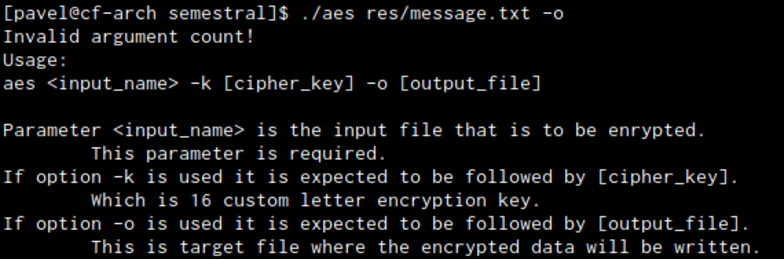
\includegraphics[width=\textwidth]{img/aes_arg_err.pdf}
	\caption{Příklad spuštění s chybějícím parametrem po přepínači -o}
	\label{fig:aes_arg_err}
\end{figure}
%
% Závěr
%
\section{Závěr}
Program by měl bez problému fungovat. Byl otestován proti výstupům
ze stránky \url{aes.online-domain-tools.com/} a vrací shodné výsledky. Program 
je také velice rychlý. Soubor o velikosti zhruba 3 MB zašifruje za\,zhruba
2.2 vteřiny a testovací soubor \textbf{Shea.jpg} kolem 0.1 vteřiny.

Pár detailů na zlepšení se ale určitě najde. Například by neškodilo zvětšit
výstupní buffer, protože momentálně má program maximální výstupní buffer 5 MiB.
Dále by určitě bylo vhodné přepsat můj \textbf{u\_char} (typedef pro
\texttt{unsigned char}) na jiný datový typ,
který má pevně danou velikost 1 Byte. Začal jsem používáním \texttt{char}, 
protože jsem ze začátku načítal soubor do bufferu typu \texttt{char}, ale
protože to způsobovalo potíže s přetékáním změnil jsem \texttt{char} na
\texttt{unsigned char}. Toto není takový problém při použití překladače gcc
a většiny překladačů, kde je char 1 Byte, ale pokud by byl použit překladač,
který bere char jako více Bytový typ nastal by problém.

Další potenciální problém, také s načítáním, je šifrování během načítání
souboru. Výhodou je, že soubor je šifrován bez závislosti na velikosti
souboru, ale nevýhodou a potenciálním nebezpečím je stream otevřený
po většinu doby běhu programu.
%
\end{document}
